\section{Introduction}

Cette manipulation a pour but la caract\'erisation d'un module optique (OM) développé pour l'expérience AMANDA. Afin d'étudier les propriétés de cet OM, vous devrez mettre au point le dispositif nécessaire à la prise de mesure. Après avoir pris connaissance avec le dispositif, vous serez ainsi amené à développer vous même la logique d'acquisition des données. Vous analyserez ensuite celles-ci grâce aux outils statistiques et informatiques que vous aurez vu en cours. 

\subsection{Rappel théorique}

\subsubsection{Rayons cosmiques}

\subsubsection{Effet Tcherenkov}

\subsubsection{Détecteur Tcherenkov}


\subsubsection{Signal type}

Nous allons à présent étudier les différentes composantes d'un spectre en charge typique de la réponse d'un photo-multiplicateur.\\

\textbf{Piédestal :} Il s'agit d'évènements sans charge qui prennent la forme d'un pic en zéro.\\

\textbf{Dark current :} Bruit associe au PM, il survient lorsqu'un électron est arraché à une dynode sans qu'un photon incident n'arrive à la photo-cathode. Il nous donne une exponentielle décroissante.\\

\textbf{Pic des photo-électrons :} Ce sont le réponse en charge du PM pour différent nombre de photo-électrons.

Le largeur de la gaussienne du premier photo-électron (1pe) va nous donner la résolution en charge du PM. La relation entre la hauteur des gaussiennes nous est donné par la distribution de Poisson.

\begin{figure}[!h]
    \center{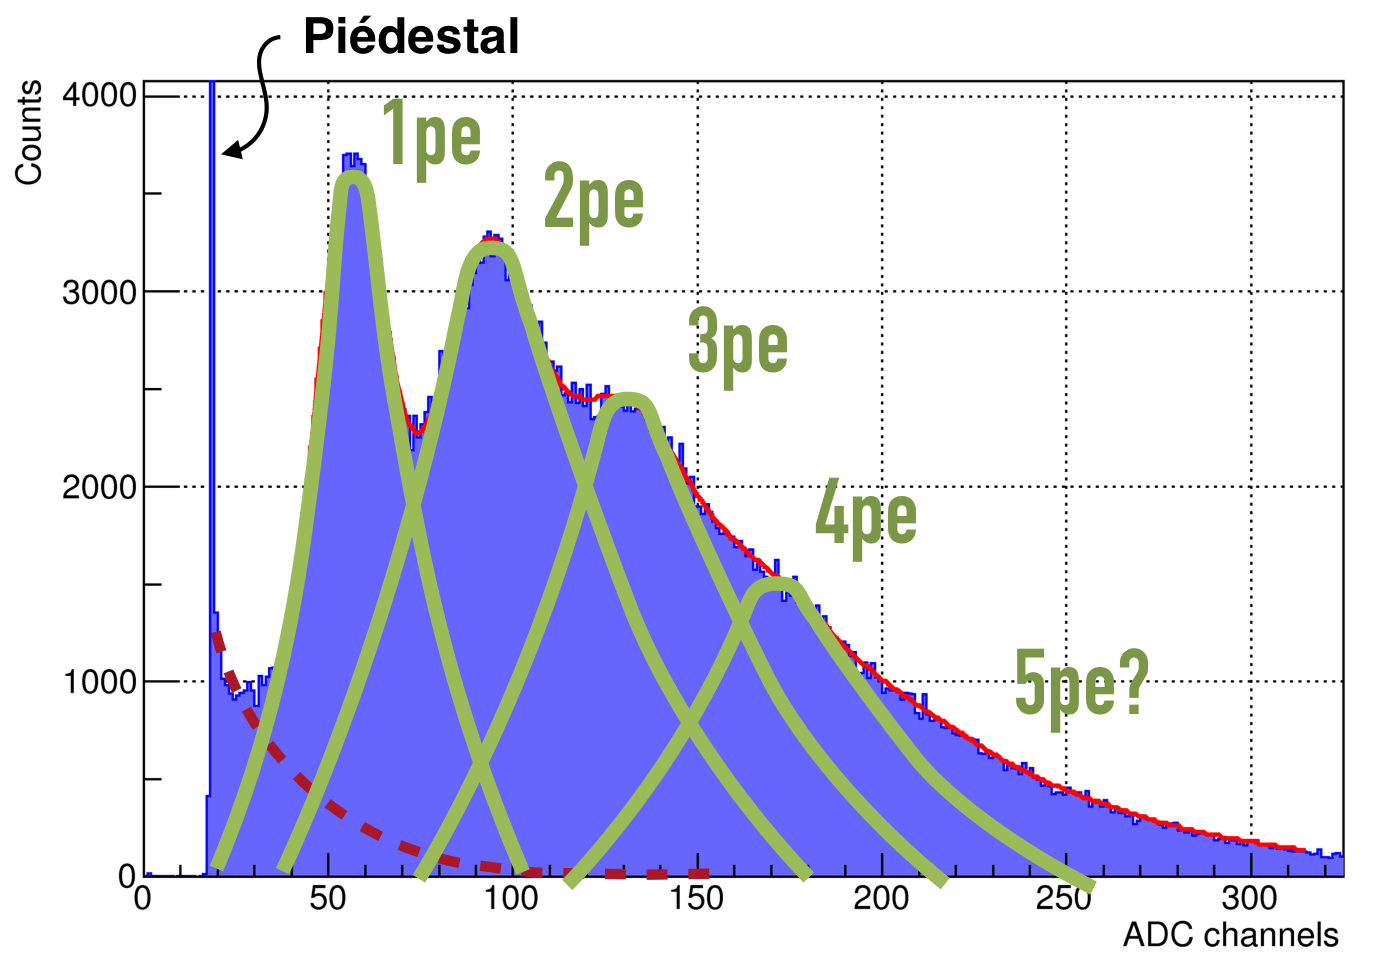
\includegraphics[width=0.7\textwidth]
    {figures/SpectreEnCharge.png}}
    \caption{\label{fig:spectre} Spectre en charge d'un photo-multiplicateur.}
\end{figure}

\subsection{Agenda du laboratoire}
\textbf{Lundi}
\begin{itemize}
\item Prendre connaissance avec le matériel
\item Vérifier le signal analogique des PMs et la sortie correspondante du discriminateur avec l'oscilloscope.
\item Implémenter de la table de vérité pour la logique d'acquisition ou trigger.
\item En utilisant les scaler NIM, calculer l’éfficacité de PM2 vs PM1 et PM3 (dispositif 2), ou PM1 vs PM2 et OM (dispositif 1) en fonction de la haute tension et du seuil du discriminateur. Mesurer aussi les taux de PM1 (PM2) en fonction de la haute sension et le seuil.
\end{itemize}
\vspace{\baselineskip}
\textbf{Mardi}
\begin{itemize}
\item Calibrer l'ADC: Introduire une charge connue à l'entrée de l’ADC. Prendre des données pour différentes charges avec le logiciel associé. Déterminer le paramètre de conversion de numéro de coups d’ADC vers charge
\item Préparer l'acquisition de données, vérifier avec l'oscilloscope que les signaux et le gate arrivent en même temps à l'ADC.
\item Démarrer l'acquisition de données avec LabView pour obternir le spectre en charge du PMT quand il y a un signal.
\end{itemize}
\vspace{\baselineskip}
\textbf{Mercredi}
\begin{itemize}
\item Construire la logique d'acquisition pour le bruit de fond.
\item Écrire la table de vérité pour définir un événement du bruit.
\item Vérifier que le gate et le signal du PMT arrivent simultanément à l'ADC.
\item Démarrer l'acquisition de données pour obtenir le spectre en charge quand il n'y a pas de signal.
\end{itemize}
\vspace{\baselineskip}
\textbf{Jeudi et Vendredi}
\begin{itemize}
\item Développement d'un programme de génération Monte Carlo d'une distribution normale et faire le fit de votre distribution Monte Carlo.
\item Développement des programmes d'analyse.
\item Dernier jour pour présenter les résultats des exercices.
\item Préparation de la présentation.
\end{itemize}

\pagebreak